% !TeX spellcheck = pt_PT
%
%
% Capitulo 5
%
\chapter{Testes} \label{testes}
Este capítulo aborda os testes executados no projeto.

\section{Aplicação Servidora} \label{sec51}
A partir desta fase do projeto, todos os testes feitos à aplicação servidora passaram a ser feitos a partir de uma \textit{framework} chamada \textit{Mockito}. Em [4] encontramos a referência para esta \textit{framework}. 

O \textit{Mockito} é uma \textit{framework Java} focada em testes unitários, que permite injetar \textit{mocks} nas classes que queremos testar, permitindo assim criar um \textit{man-in-the-middle} que intercepta chamadas a métodos dessas classes. Através da lógica \textit{when(calledMethod)} - \textit{thenReturn(desiredValue)}, podemos atribuir comportamentos aos \textit{mocks} para que quando um certo método é chamado, em vez da chamada acontecer, o \textit{mock} retorna um valor pré-fabricado. Esta \textit{framework} é especialmente útil para testar a camada de \textit{Business} da nossa aplicação servidora, sem que os testes tenham de fazer \textit{GET} ou \textit{POST} sobre a informação da base de dados.

Podemos observar, no troço de código seguinte, alguns dos testes feitos ao \textit{AthleteBusiness}:

\begin{lstlisting}
public class AthleteBusinessTest {

	@InjectMocks
	 private AthleteBusiness business;
	
	@Mock
	 AthleteRepository repository;
	
	@Mock
	 ProfileRepository profileRepository;
	
	/* . . . */
	
	@Test
	public void postProfileTest(){
		Athlete athlete = createAthlete();
		Mockito.when(repository.save(Mockito.any(Athlete.class))).thenReturn(athlete);
		Mockito.when(profileRepository.save(Mockito.any(Profile.class))).thenReturn(createProfile());
		Long id = business.postAthlete(athlete);
		Assert.assertEquals(athlete.getId(), id);
	}
	
	@Test
	public void getExistingProfileById(){
		Athlete athlete = createAthlete();
		Mockito.when(repository.findById(Mockito.any(Long.class))).thenReturn(Optional.of(athlete));
		Athlete athlete2 = business.findAthleteById(1L);
		Assert.assertEquals(athlete.getTrainingSchedules().size(), athlete2.getTrainingSchedules().size());
		Assert.assertEquals(athlete.getAthleteGameStats().size(), athlete2.getAthleteGameStats().size());
		Assert.assertEquals(athlete.getAthletePractices().size(), athlete2.getAthletePractices().size());
		Assert.assertEquals(athlete.getActiveRosters().size(), athlete2.getActiveRosters().size());
		Assert.assertEquals(athlete.getGames().size(), athlete2.getGames().size());
		Assert.assertEquals(athlete.getId(), athlete2.getId());
		Assert.assertEquals(athlete.getAthleteNumber(), athlete2.getAthleteNumber());
		Assert.assertEquals(athlete.getComment(), athlete2.getComment());
		Assert.assertEquals(athlete.getHeight(), athlete2.getHeight());
		Assert.assertEquals(athlete.getWeight(), athlete2.getWeight());
		Assert.assertEquals(athlete.getPositions(), athlete2.getPositions());
	}
	
	@Test(expected = ResourceNotFoundException.class)
		public void updateNotExistingProfile(){
		Athlete athlete = createAthlete();
		Mockito.when(repository.findById(Mockito.any(Long.class))).thenReturn(Optional.empty());
		Mockito.when(profileRepository.findById(Mockito.any(Long.class))).thenReturn(Optional.empty());
		business.updateAthlete(athlete);
	}
\end{lstlisting}

A anotação \textit{@Mock} serve para criar \textit{Mocks} que vão suportar a classe que vai ser testada (neste caso, os repositórios das entidades da classe a ser testada). A anotação \textit{@InjectMocks} cria uma instância da classe que irá ser testada.

\begin{figure}[h]
	\begin{center}
		\resizebox{120mm}{!}{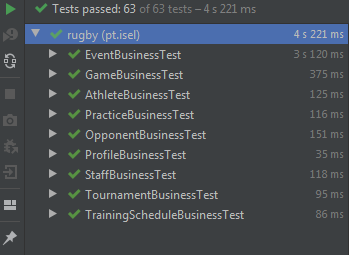
\includegraphics{./figures/tests.png}}
	\end{center}
	\caption{Demonstração de todos os testes da aplicação servidora a concluirem com sucesso.}\label{fig:gamessortednameup}
\end{figure}
\newpage
\section{Aplicação Cliente}\label{sec52}
Todos os testes feitos à aplicação cliente foram executados com ligação direta à \textit{web API} exposta pela aplicação servidora. Todos os exemplos e demonstrações apresentados ao longo do Capítulo 4 têm como base informação que provem diretamente das chamadas aos \textit{endpoints} da aplicação servidora, e toda a aplicação cliente foi testada com esses dados.